\documentclass{standalone}
\usepackage{tikz}
\usetikzlibrary{patterns, positioning}

\begin{document}
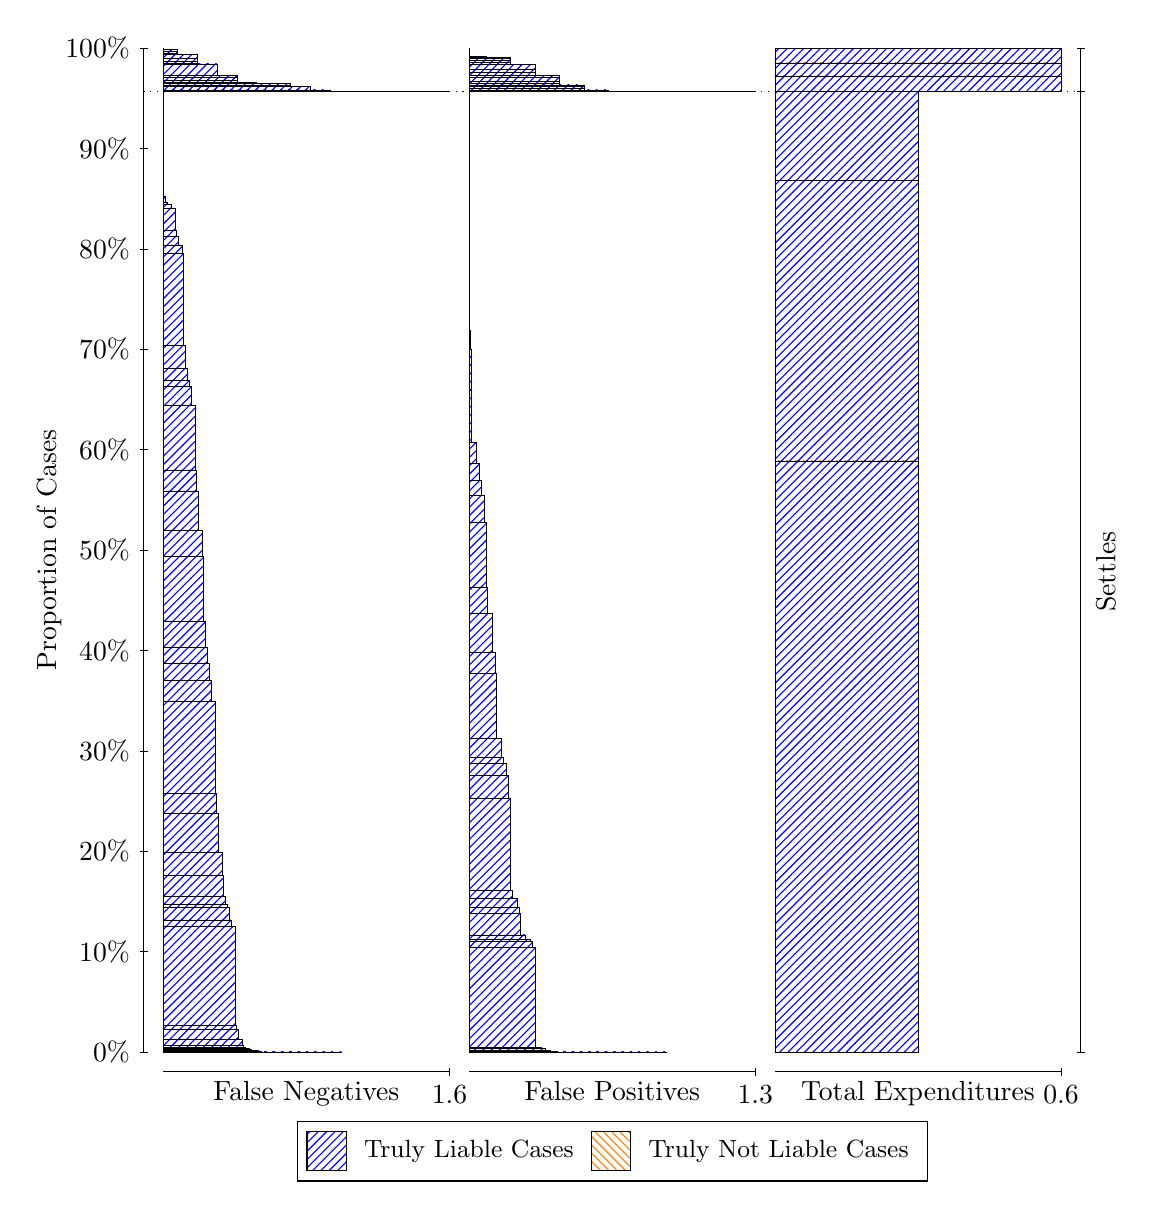
\begin{tikzpicture}
\draw[black, very thin] (1.5,1.75) -- (1.5,14.5);
\node[rotate=90, anchor=center] at (0.3, 8.125) {Proportion of Cases};
\draw[black, very thin] (1.45,1.75) -- (1.55,1.75);
\node[anchor=east] at (1.45, 1.75) {0\%};
\draw[black, very thin] (1.45,3.025) -- (1.55,3.025);
\node[anchor=east] at (1.45, 3.025) {10\%};
\draw[black, very thin] (1.45,4.3) -- (1.55,4.3);
\node[anchor=east] at (1.45, 4.3) {20\%};
\draw[black, very thin] (1.45,5.575) -- (1.55,5.575);
\node[anchor=east] at (1.45, 5.575) {30\%};
\draw[black, very thin] (1.45,6.85) -- (1.55,6.85);
\node[anchor=east] at (1.45, 6.85) {40\%};
\draw[black, very thin] (1.45,8.125) -- (1.55,8.125);
\node[anchor=east] at (1.45, 8.125) {50\%};
\draw[black, very thin] (1.45,9.4) -- (1.55,9.4);
\node[anchor=east] at (1.45, 9.4) {60\%};
\draw[black, very thin] (1.45,10.675) -- (1.55,10.675);
\node[anchor=east] at (1.45, 10.675) {70\%};
\draw[black, very thin] (1.45,11.95) -- (1.55,11.95);
\node[anchor=east] at (1.45, 11.95) {80\%};
\draw[black, very thin] (1.45,13.225) -- (1.55,13.225);
\node[anchor=east] at (1.45, 13.225) {90\%};
\draw[black, very thin] (1.45,14.5) -- (1.55,14.5);
\node[anchor=east] at (1.45, 14.5) {100\%};

\draw[black, very thin] (13.4,1.75) -- (13.4,14.5);
\draw[black, very thin] (13.35,1.75) -- (13.45,1.75);
\node[anchor=west] at (13.35, 1.75) {};
\draw[black, very thin] (13.35,13.947) -- (13.45,13.947);
\node[anchor=west] at (13.35, 13.947) {};
\draw[black, very thin] (13.35,14.5) -- (13.45,14.5);
\node[anchor=west] at (13.35, 14.5) {};

\draw[black, very thin, pattern color=blue, pattern=north east lines] (1.75,1.75) rectangle (4.0208,1.75);
\draw[black, very thin, pattern color=blue, pattern=north east lines] (1.75,1.75) rectangle (3.7937,1.75);
\draw[black, very thin, pattern color=blue, pattern=north east lines] (1.75,1.75) rectangle (3.7685,1.75);
\draw[black, very thin, pattern color=blue, pattern=north east lines] (1.75,1.75) rectangle (3.6802,1.75);
\draw[black, very thin, pattern color=blue, pattern=north east lines] (1.75,1.75) rectangle (3.5667,1.75);
\draw[black, very thin, pattern color=blue, pattern=north east lines] (1.75,1.75) rectangle (3.5414,1.75);
\draw[black, very thin, pattern color=blue, pattern=north east lines] (1.75,1.75) rectangle (3.5162,1.75);
\draw[black, very thin, pattern color=blue, pattern=north east lines] (1.75,1.75) rectangle (3.4531,1.75);
\draw[black, very thin, pattern color=blue, pattern=north east lines] (1.75,1.75) rectangle (3.4279,1.75);
\draw[black, very thin, pattern color=blue, pattern=north east lines] (1.75,1.75) rectangle (3.3396,1.75);
\draw[black, very thin, pattern color=blue, pattern=north east lines] (1.75,1.75) rectangle (3.3144,1.75);
\draw[black, very thin, pattern color=blue, pattern=north east lines] (1.75,1.75) rectangle (3.2891,1.75);
\draw[black, very thin, pattern color=blue, pattern=north east lines] (1.75,1.75) rectangle (3.2639,1.75);
\draw[black, very thin, pattern color=blue, pattern=north east lines] (1.75,1.75) rectangle (3.2008,1.7501);
\draw[black, very thin, pattern color=blue, pattern=north east lines] (1.75,1.7501) rectangle (3.1756,1.7501);
\draw[black, very thin, pattern color=blue, pattern=north east lines] (1.75,1.7501) rectangle (3.1125,1.7505);
\draw[black, very thin, pattern color=blue, pattern=north east lines] (1.75,1.7505) rectangle (3.0873,1.7511);
\draw[black, very thin, pattern color=blue, pattern=north east lines] (1.75,1.7511) rectangle (3.062,1.7511);
\draw[black, very thin, pattern color=blue, pattern=north east lines] (1.75,1.7511) rectangle (3.0368,1.7511);
\draw[black, very thin, pattern color=blue, pattern=north east lines] (1.75,1.7511) rectangle (3.0116,1.7517);
\draw[black, very thin, pattern color=blue, pattern=north east lines] (1.75,1.7517) rectangle (2.999,1.7627);
\draw[black, very thin, pattern color=blue, pattern=north east lines] (1.75,1.7627) rectangle (2.9485,1.7684);
\draw[black, very thin, pattern color=blue, pattern=north east lines] (1.75,1.7684) rectangle (2.9233,1.7708);
\draw[black, very thin, pattern color=blue, pattern=north east lines] (1.75,1.7708) rectangle (2.8602,1.7792);
\draw[black, very thin, pattern color=blue, pattern=north east lines] (1.75,1.7792) rectangle (2.835,1.8003);
\draw[black, very thin, pattern color=blue, pattern=north east lines] (1.75,1.8003) rectangle (2.8097,1.8026);
\draw[black, very thin, pattern color=blue, pattern=north east lines] (1.75,1.8026) rectangle (2.7845,1.8077);
\draw[black, very thin, pattern color=blue, pattern=north east lines] (1.75,1.8077) rectangle (2.7593,1.834);
\draw[black, very thin, pattern color=blue, pattern=north east lines] (1.75,1.834) rectangle (2.7466,1.9163);
\draw[black, very thin, pattern color=blue, pattern=north east lines] (1.75,1.9163) rectangle (2.6962,2.0329);
\draw[black, very thin, pattern color=blue, pattern=north east lines] (1.75,2.0329) rectangle (2.6709,2.0861);
\draw[black, very thin, pattern color=blue, pattern=north east lines] (1.75,2.0861) rectangle (2.6583,3.3492);
\draw[black, very thin, pattern color=blue, pattern=north east lines] (1.75,3.3492) rectangle (2.6079,3.4289);
\draw[black, very thin, pattern color=blue, pattern=north east lines] (1.75,3.4289) rectangle (2.5826,3.582);
\draw[black, very thin, pattern color=blue, pattern=north east lines] (1.75,3.582) rectangle (2.5574,3.6303);
\draw[black, very thin, pattern color=blue, pattern=north east lines] (1.75,3.6303) rectangle (2.5322,3.7254);
\draw[black, very thin, pattern color=blue, pattern=north east lines] (1.75,3.7254) rectangle (2.5069,3.9972);
\draw[black, very thin, pattern color=blue, pattern=north east lines] (1.75,3.9972) rectangle (2.4943,4.2865);
\draw[black, very thin, pattern color=blue, pattern=north east lines] (1.75,4.2865) rectangle (2.4439,4.784);
\draw[black, very thin, pattern color=blue, pattern=north east lines] (1.75,4.784) rectangle (2.4186,5.0297);
\draw[black, very thin, pattern color=blue, pattern=north east lines] (1.75,5.0297) rectangle (2.406,6.2056);
\draw[black, very thin, pattern color=blue, pattern=north east lines] (1.75,6.2056) rectangle (2.3556,6.4722);
\draw[black, very thin, pattern color=blue, pattern=north east lines] (1.75,6.4722) rectangle (2.3303,6.691);
\draw[black, very thin, pattern color=blue, pattern=north east lines] (1.75,6.691) rectangle (2.3051,6.8835);
\draw[black, very thin, pattern color=blue, pattern=north east lines] (1.75,6.8835) rectangle (2.2799,7.2212);
\draw[black, very thin, pattern color=blue, pattern=north east lines] (1.75,7.2212) rectangle (2.2546,8.0412);
\draw[black, very thin, pattern color=blue, pattern=north east lines] (1.75,8.0412) rectangle (2.242,8.3789);
\draw[black, very thin, pattern color=blue, pattern=north east lines] (1.75,8.3789) rectangle (2.1916,8.8763);
\draw[black, very thin, pattern color=blue, pattern=north east lines] (1.75,8.8763) rectangle (2.1663,9.1429);
\draw[black, very thin, pattern color=blue, pattern=north east lines] (1.75,9.1429) rectangle (2.1537,9.963);
\draw[black, very thin, pattern color=blue, pattern=north east lines] (1.75,9.963) rectangle (2.1032,10.209);
\draw[black, very thin, pattern color=blue, pattern=north east lines] (1.75,10.209) rectangle (2.078,10.283);
\draw[black, very thin, pattern color=blue, pattern=north east lines] (1.75,10.283) rectangle (2.0528,10.431);
\draw[black, very thin, pattern color=blue, pattern=north east lines] (1.75,10.431) rectangle (2.0275,10.72);
\draw[black, very thin, pattern color=blue, pattern=north east lines] (1.75,10.72) rectangle (2.0023,11.896);
\draw[black, very thin, pattern color=blue, pattern=north east lines] (1.75,11.896) rectangle (1.9897,11.991);
\draw[black, very thin, pattern color=blue, pattern=north east lines] (1.75,11.991) rectangle (1.9392,12.108);
\draw[black, very thin, pattern color=blue, pattern=north east lines] (1.75,12.108) rectangle (1.914,12.187);
\draw[black, very thin, pattern color=blue, pattern=north east lines] (1.75,12.187) rectangle (1.9014,12.459);
\draw[black, very thin, pattern color=blue, pattern=north east lines] (1.75,12.459) rectangle (1.8509,12.512);
\draw[black, very thin, pattern color=blue, pattern=north east lines] (1.75,12.512) rectangle (1.8257,12.52);
\draw[black, very thin, pattern color=blue, pattern=north east lines] (1.75,12.52) rectangle (1.8005,12.541);
\draw[black, very thin, pattern color=blue, pattern=north east lines] (1.75,12.541) rectangle (1.7752,12.623);
\draw[black, very thin, pattern color=orange, pattern=north west lines] (1.75,12.623) rectangle (1.75,12.623);
\draw[black, very thin, pattern color=blue, pattern=north east lines] (1.75,12.623) rectangle (1.75,13.947);
\draw[black, very thin, pattern color=blue, pattern=north east lines] (1.75,13.947) rectangle (5.3833,13.947);
\draw[black, very thin, pattern color=blue, pattern=north east lines] (1.75,13.947) rectangle (5.131,13.947);
\draw[black, very thin, pattern color=blue, pattern=north east lines] (1.75,13.947) rectangle (4.8787,13.947);
\draw[black, very thin, pattern color=blue, pattern=north east lines] (1.75,13.947) rectangle (4.6264,13.947);
\draw[black, very thin, pattern color=blue, pattern=north east lines] (1.75,13.947) rectangle (4.3741,13.948);
\draw[black, very thin, pattern color=blue, pattern=north east lines] (1.75,13.948) rectangle (4.1975,13.948);
\draw[black, very thin, pattern color=blue, pattern=north east lines] (1.75,13.948) rectangle (4.1218,13.949);
\draw[black, very thin, pattern color=blue, pattern=north east lines] (1.75,13.949) rectangle (4.1218,13.951);
\draw[black, very thin, pattern color=blue, pattern=north east lines] (1.75,13.951) rectangle (3.9451,13.951);
\draw[black, very thin, pattern color=blue, pattern=north east lines] (1.75,13.951) rectangle (3.9451,13.951);
\draw[black, very thin, pattern color=blue, pattern=north east lines] (1.75,13.951) rectangle (3.8694,13.969);
\draw[black, very thin, pattern color=blue, pattern=north east lines] (1.75,13.969) rectangle (3.6928,13.969);
\draw[black, very thin, pattern color=blue, pattern=north east lines] (1.75,13.969) rectangle (3.6928,13.969);
\draw[black, very thin, pattern color=blue, pattern=north east lines] (1.75,13.969) rectangle (3.6171,14.014);
\draw[black, very thin, pattern color=blue, pattern=north east lines] (1.75,14.014) rectangle (3.4405,14.014);
\draw[black, very thin, pattern color=blue, pattern=north east lines] (1.75,14.014) rectangle (3.3648,14.026);
\draw[black, very thin, pattern color=blue, pattern=north east lines] (1.75,14.026) rectangle (3.3648,14.047);
\draw[black, very thin, pattern color=blue, pattern=north east lines] (1.75,14.047) rectangle (3.1882,14.047);
\draw[black, very thin, pattern color=blue, pattern=north east lines] (1.75,14.047) rectangle (3.1125,14.052);
\draw[black, very thin, pattern color=blue, pattern=north east lines] (1.75,14.052) rectangle (2.9359,14.053);
\draw[black, very thin, pattern color=blue, pattern=north east lines] (1.75,14.053) rectangle (2.9359,14.068);
\draw[black, very thin, pattern color=blue, pattern=north east lines] (1.75,14.068) rectangle (2.8602,14.068);
\draw[black, very thin, pattern color=blue, pattern=north east lines] (1.75,14.068) rectangle (2.6836,14.068);
\draw[black, very thin, pattern color=blue, pattern=north east lines] (1.75,14.068) rectangle (2.6836,14.088);
\draw[black, very thin, pattern color=blue, pattern=north east lines] (1.75,14.088) rectangle (2.6836,14.126);
\draw[black, very thin, pattern color=blue, pattern=north east lines] (1.75,14.126) rectangle (2.6836,14.155);
\draw[black, very thin, pattern color=blue, pattern=north east lines] (1.75,14.155) rectangle (2.6079,14.155);
\draw[black, very thin, pattern color=blue, pattern=north east lines] (1.75,14.155) rectangle (2.4312,14.157);
\draw[black, very thin, pattern color=blue, pattern=north east lines] (1.75,14.157) rectangle (2.4312,14.298);
\draw[black, very thin, pattern color=blue, pattern=north east lines] (1.75,14.298) rectangle (2.3556,14.298);
\draw[black, very thin, pattern color=blue, pattern=north east lines] (1.75,14.298) rectangle (2.1789,14.311);
\draw[black, very thin, pattern color=blue, pattern=north east lines] (1.75,14.311) rectangle (2.1789,14.328);
\draw[black, very thin, pattern color=blue, pattern=north east lines] (1.75,14.328) rectangle (2.1789,14.372);
\draw[black, very thin, pattern color=blue, pattern=north east lines] (1.75,14.372) rectangle (2.1789,14.416);
\draw[black, very thin, pattern color=blue, pattern=north east lines] (1.75,14.416) rectangle (2.1032,14.416);
\draw[black, very thin, pattern color=blue, pattern=north east lines] (1.75,14.416) rectangle (1.9266,14.437);
\draw[black, very thin, pattern color=blue, pattern=north east lines] (1.75,14.437) rectangle (1.9266,14.464);
\draw[black, very thin, pattern color=blue, pattern=north east lines] (1.75,14.464) rectangle (1.9266,14.478);
\draw[black, very thin, pattern color=orange, pattern=north west lines] (1.75,14.478) rectangle (1.75,14.478);
\draw[black, very thin, pattern color=blue, pattern=north east lines] (1.75,14.478) rectangle (1.75,14.5);
\draw[black, very thin, pattern color=orange, pattern=north west lines] (5.6333,1.75) rectangle (8.1487,1.75);
\draw[black, very thin, pattern color=blue, pattern=north east lines] (5.6333,1.75) rectangle (8.1487,1.75);
\draw[black, very thin, pattern color=blue, pattern=north east lines] (5.6333,1.75) rectangle (7.8382,1.75);
\draw[black, very thin, pattern color=orange, pattern=north west lines] (5.6333,1.75) rectangle (7.7295,1.75);
\draw[black, very thin, pattern color=blue, pattern=north east lines] (5.6333,1.75) rectangle (7.7295,1.75);
\draw[black, very thin, pattern color=orange, pattern=north west lines] (5.6333,1.75) rectangle (7.5897,1.75);
\draw[black, very thin, pattern color=blue, pattern=north east lines] (5.6333,1.75) rectangle (7.5897,1.75);
\draw[black, very thin, pattern color=blue, pattern=north east lines] (5.6333,1.75) rectangle (7.5276,1.75);
\draw[black, very thin, pattern color=blue, pattern=north east lines] (5.6333,1.75) rectangle (7.4189,1.75);
\draw[black, very thin, pattern color=orange, pattern=north west lines] (5.6333,1.75) rectangle (7.3103,1.75);
\draw[black, very thin, pattern color=blue, pattern=north east lines] (5.6333,1.75) rectangle (7.3103,1.75);
\draw[black, very thin, pattern color=blue, pattern=north east lines] (5.6333,1.75) rectangle (7.2792,1.75);
\draw[black, very thin, pattern color=blue, pattern=north east lines] (5.6333,1.75) rectangle (7.2171,1.75);
\draw[black, very thin, pattern color=orange, pattern=north west lines] (5.6333,1.75) rectangle (7.1705,1.75);
\draw[black, very thin, pattern color=blue, pattern=north east lines] (5.6333,1.75) rectangle (7.1705,1.75);
\draw[black, very thin, pattern color=blue, pattern=north east lines] (5.6333,1.75) rectangle (7.1084,1.75);
\draw[black, very thin, pattern color=orange, pattern=north west lines] (5.6333,1.75) rectangle (7.0308,1.75);
\draw[black, very thin, pattern color=blue, pattern=north east lines] (5.6333,1.75) rectangle (7.0308,1.75);
\draw[black, very thin, pattern color=blue, pattern=north east lines] (5.6333,1.75) rectangle (6.9997,1.75);
\draw[black, very thin, pattern color=blue, pattern=north east lines] (5.6333,1.75) rectangle (6.9687,1.75);
\draw[black, very thin, pattern color=blue, pattern=north east lines] (5.6333,1.75) rectangle (6.9066,1.7506);
\draw[black, very thin, pattern color=orange, pattern=north west lines] (5.6333,1.7506) rectangle (6.891,1.7506);
\draw[black, very thin, pattern color=blue, pattern=north east lines] (5.6333,1.7506) rectangle (6.891,1.751);
\draw[black, very thin, pattern color=blue, pattern=north east lines] (5.6333,1.751) rectangle (6.86,1.751);
\draw[black, very thin, pattern color=blue, pattern=north east lines] (5.6333,1.751) rectangle (6.7979,1.7511);
\draw[black, very thin, pattern color=orange, pattern=north west lines] (5.6333,1.7511) rectangle (6.7513,1.7511);
\draw[black, very thin, pattern color=blue, pattern=north east lines] (5.6333,1.7511) rectangle (6.7513,1.7621);
\draw[black, very thin, pattern color=blue, pattern=north east lines] (5.6333,1.7621) rectangle (6.7202,1.7627);
\draw[black, very thin, pattern color=blue, pattern=north east lines] (5.6333,1.7627) rectangle (6.6892,1.763);
\draw[black, very thin, pattern color=blue, pattern=north east lines] (5.6333,1.763) rectangle (6.6581,1.7654);
\draw[black, very thin, pattern color=blue, pattern=north east lines] (5.6333,1.7654) rectangle (6.596,1.7916);
\draw[black, very thin, pattern color=blue, pattern=north east lines] (5.6333,1.7916) rectangle (6.5805,1.8001);
\draw[black, very thin, pattern color=blue, pattern=north east lines] (5.6333,1.8001) rectangle (6.5494,1.8058);
\draw[black, very thin, pattern color=blue, pattern=north east lines] (5.6333,1.8058) rectangle (6.4873,1.8109);
\draw[black, very thin, pattern color=orange, pattern=north west lines] (5.6333,1.8109) rectangle (6.4718,1.8109);
\draw[black, very thin, pattern color=blue, pattern=north east lines] (5.6333,1.8109) rectangle (6.4718,3.0741);
\draw[black, very thin, pattern color=blue, pattern=north east lines] (5.6333,3.0741) rectangle (6.4407,3.1563);
\draw[black, very thin, pattern color=blue, pattern=north east lines] (5.6333,3.1563) rectangle (6.4097,3.1771);
\draw[black, very thin, pattern color=blue, pattern=north east lines] (5.6333,3.1771) rectangle (6.3786,3.1848);
\draw[black, very thin, pattern color=blue, pattern=north east lines] (5.6333,3.1848) rectangle (6.3476,3.2381);
\draw[black, very thin, pattern color=blue, pattern=north east lines] (5.6333,3.2381) rectangle (6.2855,3.5099);
\draw[black, very thin, pattern color=blue, pattern=north east lines] (5.6333,3.5099) rectangle (6.2699,3.5896);
\draw[black, very thin, pattern color=blue, pattern=north east lines] (5.6333,3.5896) rectangle (6.2389,3.7062);
\draw[black, very thin, pattern color=blue, pattern=north east lines] (5.6333,3.7062) rectangle (6.1768,3.8012);
\draw[black, very thin, pattern color=blue, pattern=north east lines] (5.6333,3.8012) rectangle (6.1613,4.9771);
\draw[black, very thin, pattern color=blue, pattern=north east lines] (5.6333,4.9771) rectangle (6.1302,5.2664);
\draw[black, very thin, pattern color=blue, pattern=north east lines] (5.6333,5.2664) rectangle (6.0991,5.414);
\draw[black, very thin, pattern color=blue, pattern=north east lines] (5.6333,5.414) rectangle (6.0681,5.4886);
\draw[black, very thin, pattern color=blue, pattern=north east lines] (5.6333,5.4886) rectangle (6.037,5.7343);
\draw[black, very thin, pattern color=blue, pattern=north east lines] (5.6333,5.7343) rectangle (5.9749,6.5544);
\draw[black, very thin, pattern color=blue, pattern=north east lines] (5.6333,6.5544) rectangle (5.9594,6.821);
\draw[black, very thin, pattern color=blue, pattern=north east lines] (5.6333,6.821) rectangle (5.9283,7.3184);
\draw[black, very thin, pattern color=blue, pattern=north east lines] (5.6333,7.3184) rectangle (5.8662,7.6561);
\draw[black, very thin, pattern color=blue, pattern=north east lines] (5.6333,7.6561) rectangle (5.8507,8.4761);
\draw[black, very thin, pattern color=blue, pattern=north east lines] (5.6333,8.4761) rectangle (5.8197,8.8138);
\draw[black, very thin, pattern color=blue, pattern=north east lines] (5.6333,8.8138) rectangle (5.7886,9.0063);
\draw[black, very thin, pattern color=blue, pattern=north east lines] (5.6333,9.0063) rectangle (5.7575,9.2251);
\draw[black, very thin, pattern color=blue, pattern=north east lines] (5.6333,9.2251) rectangle (5.7265,9.4917);
\draw[black, very thin, pattern color=blue, pattern=north east lines] (5.6333,9.4917) rectangle (5.6644,10.668);
\draw[black, very thin, pattern color=blue, pattern=north east lines] (5.6333,10.668) rectangle (5.6489,10.913);
\draw[black, very thin, pattern color=blue, pattern=north east lines] (5.6333,10.913) rectangle (5.6333,13.947);
\draw[black, very thin, pattern color=orange, pattern=north west lines] (5.6333,13.947) rectangle (9.2667,13.947);
\draw[black, very thin, pattern color=blue, pattern=north east lines] (5.6333,13.947) rectangle (9.2667,13.947);
\draw[black, very thin, pattern color=orange, pattern=north west lines] (5.6333,13.947) rectangle (8.9561,13.947);
\draw[black, very thin, pattern color=blue, pattern=north east lines] (5.6333,13.947) rectangle (8.9561,13.947);
\draw[black, very thin, pattern color=blue, pattern=north east lines] (5.6333,13.947) rectangle (8.6456,13.947);
\draw[black, very thin, pattern color=orange, pattern=north west lines] (5.6333,13.947) rectangle (8.6456,13.947);
\draw[black, very thin, pattern color=blue, pattern=north east lines] (5.6333,13.947) rectangle (8.6456,13.947);
\draw[black, very thin, pattern color=blue, pattern=north east lines] (5.6333,13.947) rectangle (8.335,13.947);
\draw[black, very thin, pattern color=blue, pattern=north east lines] (5.6333,13.947) rectangle (8.335,13.947);
\draw[black, very thin, pattern color=orange, pattern=north west lines] (5.6333,13.947) rectangle (8.335,13.947);
\draw[black, very thin, pattern color=blue, pattern=north east lines] (5.6333,13.947) rectangle (8.335,13.947);
\draw[black, very thin, pattern color=orange, pattern=north west lines] (5.6333,13.947) rectangle (8.0245,13.947);
\draw[black, very thin, pattern color=blue, pattern=north east lines] (5.6333,13.947) rectangle (8.0245,13.948);
\draw[black, very thin, pattern color=blue, pattern=north east lines] (5.6333,13.948) rectangle (8.0245,13.948);
\draw[black, very thin, pattern color=blue, pattern=north east lines] (5.6333,13.948) rectangle (8.0245,13.948);
\draw[black, very thin, pattern color=orange, pattern=north west lines] (5.6333,13.948) rectangle (7.714,13.948);
\draw[black, very thin, pattern color=blue, pattern=north east lines] (5.6333,13.948) rectangle (7.714,13.95);
\draw[black, very thin, pattern color=blue, pattern=north east lines] (5.6333,13.95) rectangle (7.714,13.951);
\draw[black, very thin, pattern color=blue, pattern=north east lines] (5.6333,13.951) rectangle (7.4034,13.958);
\draw[black, very thin, pattern color=orange, pattern=north west lines] (5.6333,13.958) rectangle (7.4034,13.958);
\draw[black, very thin, pattern color=blue, pattern=north east lines] (5.6333,13.958) rectangle (7.4034,13.969);
\draw[black, very thin, pattern color=blue, pattern=north east lines] (5.6333,13.969) rectangle (7.0929,13.983);
\draw[black, very thin, pattern color=blue, pattern=north east lines] (5.6333,13.983) rectangle (7.0929,14.011);
\draw[black, very thin, pattern color=orange, pattern=north west lines] (5.6333,14.011) rectangle (7.0929,14.011);
\draw[black, very thin, pattern color=blue, pattern=north east lines] (5.6333,14.011) rectangle (7.0929,14.031);
\draw[black, very thin, pattern color=orange, pattern=north west lines] (5.6333,14.031) rectangle (6.8755,14.031);
\draw[black, very thin, pattern color=blue, pattern=north east lines] (5.6333,14.031) rectangle (6.8755,14.031);
\draw[black, very thin, pattern color=blue, pattern=north east lines] (5.6333,14.031) rectangle (6.7823,14.051);
\draw[black, very thin, pattern color=blue, pattern=north east lines] (5.6333,14.051) rectangle (6.7823,14.077);
\draw[black, very thin, pattern color=blue, pattern=north east lines] (5.6333,14.077) rectangle (6.7823,14.13);
\draw[black, very thin, pattern color=blue, pattern=north east lines] (5.6333,14.13) rectangle (6.7823,14.132);
\draw[black, very thin, pattern color=blue, pattern=north east lines] (5.6333,14.132) rectangle (6.7823,14.15);
\draw[black, very thin, pattern color=orange, pattern=north west lines] (5.6333,14.15) rectangle (6.565,14.15);
\draw[black, very thin, pattern color=blue, pattern=north east lines] (5.6333,14.15) rectangle (6.565,14.15);
\draw[black, very thin, pattern color=blue, pattern=north east lines] (5.6333,14.15) rectangle (6.4718,14.195);
\draw[black, very thin, pattern color=blue, pattern=north east lines] (5.6333,14.195) rectangle (6.4718,14.227);
\draw[black, very thin, pattern color=blue, pattern=north east lines] (5.6333,14.227) rectangle (6.4718,14.292);
\draw[black, very thin, pattern color=orange, pattern=north west lines] (5.6333,14.292) rectangle (6.2544,14.292);
\draw[black, very thin, pattern color=blue, pattern=north east lines] (5.6333,14.292) rectangle (6.2544,14.292);
\draw[black, very thin, pattern color=blue, pattern=north east lines] (5.6333,14.292) rectangle (6.1613,14.319);
\draw[black, very thin, pattern color=blue, pattern=north east lines] (5.6333,14.319) rectangle (6.1613,14.34);
\draw[black, very thin, pattern color=blue, pattern=north east lines] (5.6333,14.34) rectangle (6.1613,14.366);
\draw[black, very thin, pattern color=blue, pattern=north east lines] (5.6333,14.366) rectangle (6.1613,14.379);
\draw[black, very thin, pattern color=orange, pattern=north west lines] (5.6333,14.379) rectangle (5.9439,14.379);
\draw[black, very thin, pattern color=blue, pattern=north east lines] (5.6333,14.379) rectangle (5.9439,14.379);
\draw[black, very thin, pattern color=blue, pattern=north east lines] (5.6333,14.379) rectangle (5.8507,14.387);
\draw[black, very thin, pattern color=blue, pattern=north east lines] (5.6333,14.387) rectangle (5.8507,14.395);
\draw[black, very thin, pattern color=orange, pattern=north west lines] (5.6333,14.395) rectangle (5.6333,14.395);
\draw[black, very thin, pattern color=blue, pattern=north east lines] (5.6333,14.395) rectangle (5.6333,14.5);
\draw[black, very thin, pattern color=orange, pattern=north west lines] (9.5167,1.75) rectangle (11.333,1.75);
\draw[black, very thin, pattern color=blue, pattern=north east lines] (9.5167,1.75) rectangle (11.333,9.2569);
\draw[black, very thin, pattern color=orange, pattern=north west lines] (9.5167,9.2569) rectangle (11.333,9.2569);
\draw[black, very thin, pattern color=blue, pattern=north east lines] (9.5167,9.2569) rectangle (11.333,12.815);
\draw[black, very thin, pattern color=orange, pattern=north west lines] (9.5167,12.815) rectangle (11.333,12.815);
\draw[black, very thin, pattern color=blue, pattern=north east lines] (9.5167,12.815) rectangle (11.333,13.947);
\draw[black, very thin, pattern color=orange, pattern=north west lines] (9.5167,13.947) rectangle (13.15,13.947);
\draw[black, very thin, pattern color=blue, pattern=north east lines] (9.5167,13.947) rectangle (13.15,14.147);
\draw[black, very thin, pattern color=orange, pattern=north west lines] (9.5167,14.147) rectangle (13.15,14.147);
\draw[black, very thin, pattern color=blue, pattern=north east lines] (9.5167,14.147) rectangle (13.15,14.311);
\draw[black, very thin, pattern color=orange, pattern=north west lines] (9.5167,14.311) rectangle (13.15,14.311);
\draw[black, very thin, pattern color=blue, pattern=north east lines] (9.5167,14.311) rectangle (13.15,14.5);
\draw[black, dotted] (1.5,13.947) -- (13.4,13.947);
\draw[black, very thin] (1.75,1.5) -- (5.3833,1.5);
\node[anchor=north] at (3.5667, 1.5) {False Negatives};
\draw[black, very thin] (5.3833,1.45) -- (5.3833,1.55);
\node[anchor=north] at (5.3833, 1.45) {1.6};

\draw[black, very thin] (5.6333,1.5) -- (9.2667,1.5);
\node[anchor=north] at (7.45, 1.5) {False Positives};
\draw[black, very thin] (9.2667,1.45) -- (9.2667,1.55);
\node[anchor=north] at (9.2667, 1.45) {1.3};

\draw[black, very thin] (9.5167,1.5) -- (13.15,1.5);
\node[anchor=north] at (11.333, 1.5) {Total Expenditures};
\draw[black, very thin] (13.15,1.45) -- (13.15,1.55);
\node[anchor=north] at (13.15, 1.45) {0.6};

\node[black, centered, rotate=90] at (13.72, 7.8486) {Settles};


\draw (7.449999999999999,1.5) node[draw=none] (baseCoordinate) {};
\begin{scope}[align=center]
        \matrix[scale=0.5, draw=black, below=0.5cm of baseCoordinate, nodes={draw}, column sep=0.1cm]{
            \node[rectangle, draw, minimum width=0.5cm, minimum height=0.5cm, pattern=north east lines, pattern color=blue] {}; &
            \node[draw=none, font=\small] (B) {Truly Liable Cases}; &
            \node[rectangle, draw, minimum width=0.5cm, minimum height=0.5cm, pattern=north west lines, pattern color=orange] {}; &
            \node[draw=none, font=\small] (B) {Truly Not Liable Cases}; \\
            };
\end{scope}

\end{tikzpicture}
\end{document}